\section{The mechanism}\label{sec:mech}

The construction follows the handle-packing scheme of \cite{OpenAI2026}. In dimension four the model is
the disc bundle of degree $9$ over a cubic curve $E\subset\CP^2$ from Biran's decomposition \cite{Biran2001}
(\S\ref{sec:intro-mechanism}): its fibres are discs of capacity $\frac13$, the base area at fibre moment $p$ is
$3(1-3p)$, and the total volume is $\frac12=\vol\CP^2$. The fibre capacity gives the condition $3c_i<C$, and the
total volume gives the volume budget. The higher-dimensional models replace $E$ by a compact piece of an affine curve
and the fibre disc by $\C^{n-1}$. In each case the construction has three inputs: a model with a positive base-area
profile, a comparison on the moment polytope, and a symplectic transfer to the target. The comparison moves area
between fibre levels, and the handle turns the comparison inequality into disjoint ball embeddings. Throughout,
$n\ge2$, $m=n-1$, and the target capacity is normalised to one; the general target is recovered by the dilation of
Definition~\ref{def:ham-normalise}.

\subsection{Toric balls and area profiles}\label{sec:mech-toric}

On $\C^m$ let $p_j=\pi|w_j|^2$, $|p|=\sum_jp_j$ and
$\omega_V=\sum_jdx_j\wedge dy_j$. Away from the coordinate axes this is
$\sum_jdp_j\wedge d\theta_j$, with each angle of period one. A downward polytope is
\[
 \Delta=\{p\in\R^m_{\ge0}:\langle b_\nu,p\rangle\le\ell_\nu,\ 1\le\nu\le N\},
 \qquad b_\nu\in\R^m_{\ge0},\quad \ell_\nu>0.
\]
Write $V_\Delta=\{w:p(w)\in\Delta\}$. The equalities
$\langle b_\nu,p\rangle=\ell_\nu$ define its outer faces, and $\tau_\Delta\Delta$,
$0<\tau_\Delta<1$, is the core used to keep the source caps away from those faces.

\begin{definition}[Toric ball]\label{def:mech-toric-ball}
\lean{OAI.PackingSufficiencySupport.closedBall,
OAI.PackingSufficiencySupport.Hamiltonian.splitCapacityBall,
OAI.PackingSufficiencySupport.Hamiltonian.complexSplitPhase_capacity}
In $\C^n=\C\times\C^m$, put $\varpi=\pi|z_{\rm b}|^2$. The ball of capacity $a$ is
$B(a)=\{\varpi+|p|\le a\}$. At a fibre point with $|p|\le a$, its base slice is a disc of capacity $a-|p|$; its slice height is $0$ for $|p|>a$. Thus the slice-height function is $(a-|p|)_+$.
\end{definition}

\begin{lemma}[The cap integral]\label{lem:mech-toric-volume}
\lean{OAI.PackingSufficiencySupport.integral_simplex_tent, OAI.PackingSufficiencySupport.integral_tent}
For $a\ge0$,
\[
 \int_{\R^m_{\ge0}}(a-|p|)_+\,dp=\frac{a^{m+1}}{(m+1)!}.
\]
\end{lemma}
\begin{proof}
The simplex $\{|p|\le t\}$ has measure $t^m/m!$. Integrating its distribution function against
$(a-t)_+$ gives the displayed identity; equivalently, integrate one coordinate at a time.
\end{proof}

For each higher-dimensional model, let $\Sigma_\ell$ be its compact affine core, let
$\Gamma_{\rm phys}(p)$ be the horizontal primitive given in its model section, and put
$\kappa(p)=d_\Sigma\Gamma_{\rm phys}(p)$. The physical form on the model is
$\Omega=\omega_V+d\Gamma_{\rm phys}$. The base profile and its moment budget are
\begin{equation}\label{eq:mech-model-volume}
 \Hb(p)=\int_{\Sigma_\ell}\kappa(p),\qquad
 \mathcal B_\Delta=\int_\Delta\Hb(p)\,dp .
\end{equation}
The first integral is the intrinsic integral of the physical base curvature; the model sections give
its formula, or a uniform bound for its distance from an explicit limiting profile. The packing proof uses this
scalar budget only through the comparison inequality below.

The four-dimensional periodic model has profile $\Hb(p)=3(1-3p)$ on $[0,h]$, $h<1/3$, and
\[
 \mathcal B_{[0,h]}=3h-\frac92h^2\longrightarrow\frac12\qquad(h\uparrow1/3).
\]
Its periodic coordinates and deck maps are given in \Sref{Section}{sec:cub}.

\subsection{Why stacking fails}\label{sec:mech-stacking}

Choose auxiliary capacities $a_i$ larger than the given capacities, with
$\{|p|\le a_i\}\subset\tau_\Delta\Delta$. Placing their base discs side by side would require the
pointwise inequality $\sum_i(a_i-|p|)_+<\Hb(p)$. Set
\[
 \Pb(p)=\Hb(p)-\sum_i(a_i-|p|)_+ .
\]
The cap integral gives the exact scalar balance
\begin{equation}\label{eq:mech-mean}
 \int_\Delta\Pb=\mathcal B_\Delta-\sum_i\frac{a_i^n}{n!}.
\end{equation}
A positive integral leaves room for a comparison, but does not give the pointwise inequality required by
stacking. For example, in the periodic cubic model take $k\ge10$, $t_0\in(0,1)$, $a_i=t_0/\sqrt k$ and $h=t_0/3$.
Then $\int_0^h\Pb=t_0(1-t_0)>0$, whereas $\Pb(0)=3-\sqrt k\,t_0<0$ whenever
$t_0>3/\sqrt k$ (Figure~\ref{fig:intro-profile}). The handle construction uses the positive integral
without requiring $\Pb$ to be positive everywhere.

\subsection{The twist moves area}\label{sec:mech-twist}

Fix the model's annulus, with coordinates $(s,v)\in[0,1]\times\R/\Z$, and its compactly supported
closed one-form $\beta=b(v)\,dv$, where $b\ge0$ and $\int_0^1b=1$. Three further objects enter, each defined
in Section~\ref{sec:hdl}. The handle data include a positive reference area form $\Lambda$ on the base
(Definition~\ref{def:hdl-handle-data}(d)). The comparison datum below carries, besides its gap $\gamma$, a
reserve $\gamma_*$ with $0<\gamma_*\le\gamma$; it is the part of the gap set aside for the normalisation.
From these, \eqref{eq:hdl-eh} fixes a constant $e_\Lambda>0$, and the first Moser path of \S\ref{sec:hdl-first}
replaces the physical curvature, on the annulus, by the background $e_\Lambda\Lambda$ plus the base mass $H^*(p)\ge0$
carried by $\beta$:
\[
 \omega_V+e_\Lambda\Lambda+d\big(f(s)H^*(p)\beta\big),\qquad f=S,\qquad H^*(p)\ge\Hb(p)-\gamma_*/16
\]
(equations~\eqref{eq:hdl-ksm} and~\eqref{eq:hdl-budget}). This reserve rule and the clock $f=S$ are those of
dimension $2n\ge6$. In dimension four the budget is set directly: the handle mass is $H^*=\Hb-e_h$ with
$e_h=g/16$, the comparison gap is $\frac{31}{32}g$, the clock is $f(s)=S(2s-\frac12)$ in the handle coordinate $s$,
and the residual stays above $\frac78g$ (\Sref{Lemma}{lem:shd4-budget}); this budget replaces the
higher-dimensional reserve rule $\gamma_*\le\gamma$.

Let $q_t$ be the comparator's Hamiltonian isotopy of the fibres, $q=q_1$. The suspension
$\mathcal D_\lambda(s,v,w)=(s,v,q_{\lambda f(s)}w)$ inserts this isotopy across the annulus.
For a smooth function $K$ of the moments, put $J=K-H^*$. Adding the globally defined form
$d(J(p)\beta)$ changes only toric mixed terms away from the annulus. After the twist, the amount
available across the annulus at $w$ is
\begin{equation}\label{eq:mech-available}
 K\big(p(q^{-1}w)\big)-J\big(p(w)\big)
 =H^*\big(p(w)\big)+K\big(p(q^{-1}w)\big)-K\big(p(w)\big).
\end{equation}
The comparison supplies, for a minorant $P\le\Pb$,
\begin{equation}\label{eq:mech-comparison}
 (K-P)\big(p(qw)\big)\le K\big(p(w)\big)-\gamma\qquad(w\in V_\Delta),
 \qquad 0<\gamma_*\le\gamma.
\end{equation}
For $n\ge3$, applied at $q^{-1}w$, together with $P\le\Pb$ and $H^*\ge\Hb-\gamma_*/16$, it shows that the available amount
exceeds $\sum_i(a_i-|p(w)|)_+$ by at least $\gamma-\gamma_*/16>0$. This amount is divided among the ball layers and a
final residual layer, and the non-toric dependence on $w$ is confined to the residual layer.

In dimension four the identity~\eqref{eq:mech-available} can be read off directly. The fibre is a disc
$\bar D(h)\subset\C$ with moment $p=\pi|w|^2$, and over the annulus every form in the construction has the shape
$\omega_V+e_\Lambda\Lambda+d(G\beta)$ for a function $G(s,w)$ independent of $v$. By Lemma~\ref{lem:hdl-top-power}(b) its
restriction to the annulus through a fixed fibre point $w$ is $e_\Lambda\Lambda+\partial_sG\,ds\wedge\beta$, so, apart from
the background $e_\Lambda\Lambda$, the area above $w$ is
\[
 \int_0^1\!\!\int_0^1\partial_sG(s,w)\,b(v)\,dv\,ds=G(1,w)-G(0,w),
\]
the increase of the $\beta$-coefficient across the annulus. After the first path $G=f(s)H^*(p(w))$, so the annulus
carries $H^*(p(w))$ above every $w$. The twist $\mathcal D$ is the identity for $s\le0$ and is $(s,v,w)\mapsto(s,v,qw)$
for $s\ge1$. Write the twisted form in the coordinates of the image of $\mathcal D$ and add $d(J(p)\beta)$, which
is defined on the whole model because $p$ and $\beta$ are. Below the annulus the coefficient is $J(p(w))$. Above
it the point $w$ is the image of $z=q^{-1}w$, where the untwisted coefficient is $H^*(p(z))+J(p(z))=K(p(z))$. So the
coefficient rises from $J(p(w))$ to $K(p(q^{-1}w))$, which is~\eqref{eq:mech-available}. The \emph{layers} are $k+1$
disjoint subintervals $I_1,\dots,I_k,I_*$ of $s\in(0,1)$ (Figure~\ref{fig:mech-layers}). Across $I_i$ the
coefficient rises by a smooth cap $h_i(p(w))$, an explicit smoothing of the tent $(a_i-p)_+$, lying below the tent
for $2n\ge6$ and above it by a controlled amount in dimension four; it is the base area
needed above $w$ by a ball of capacity slightly less than $a_i$, and since on $I_i$ the form is toric, such a ball
is placed there in product form. Across the last interval $I_*$ the coefficient rises by the remainder $R^*(w)$,
which is positive because the gap $\gamma$ in~\eqref{eq:mech-comparison} exceeds the smoothing errors; it is the
only layer coefficient that depends on $w$ through more than $p(w)$.

\begin{figure}[ht]
\centering
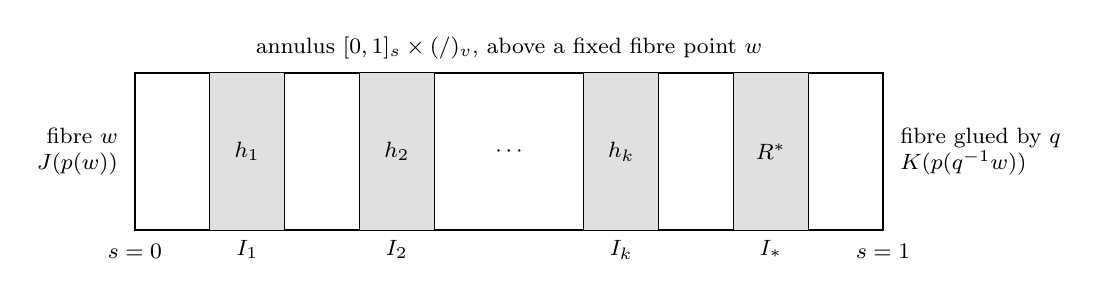
\begin{tikzpicture}[x=0.95cm,y=1cm,font=\footnotesize]
 \draw[thick] (0,0) rectangle (10,2);
 \foreach \l/\r/\t in {1/2/{h_1},3/4/{h_2},6/7/{h_k},8/9/{R^*}} {
  \fill[black!12] (\l,0) rectangle (\r,2);
  \draw (\l,0) -- (\l,2); \draw (\r,0) -- (\r,2);
  \node at ({(\l+\r)/2},1) {$\t$};
 }
 \node at (5,1) {$\cdots$};
 \node[below] at (1.5,0) {$I_1$}; \node[below] at (3.5,0) {$I_2$};
 \node[below] at (6.5,0) {$I_k$}; \node[below] at (8.5,0) {$I_*$};
 \node[below] at (0,-0.05) {$s=0$}; \node[below] at (10,-0.05) {$s=1$};
 \node[left,align=right] at (-0.1,1) {fibre $w$\\$J(p(w))$};
 \node[right,align=left] at (10.1,1) {fibre glued by $q$\\$K(p(q^{-1}w))$};
 \node[above] at (5,2.05) {annulus $[0,1]_s\times(\R/\Z)_v$, above a fixed fibre point $w$};
\end{tikzpicture}
\caption{The annulus above a fibre point $w$ in dimension four. The $\beta$-coefficient rises from $J(p(w))$ to
$K(p(q^{-1}w))$; across the layer $I_i$ it rises by the cap $h_i(p(w))$ of the $i$-th ball and across $I_*$ by the
positive remainder $R^*(w)$.}
\label{fig:mech-layers}
\end{figure}

The general comparator is constructed from a concave piecewise affine minorant $P$ with positive mean.
For its finite fixed-point construction choose
\begin{equation}\label{eq:mech-necessary}
 0<d<\min\bigl(\bar P,\beta_P\bigr),\qquad
 \bar P=|\Delta|^{-1}\int_\Delta P,
\end{equation}
where $P\ge\beta_P>0$ off the core $\tau_\Delta\Delta$. Section~\ref{sec:cmp} constructs $K$ and $q_t$ and accounts for
all approximation errors in the retained gap. The increasing rearrangements act on the moment
polytope, and their Hamiltonian realisations act on the fibres. For the equal-ball four-dimensional
case with $k\ge10$ and $\frac34<\rho\sqrt k<1$, the linear comparison of Proposition~\ref{prop:cmp-linear} gives the datum directly.

\subsection{Model, comparison datum and transfer}\label{sec:mech-interfaces}

\begin{definition}[Model input]\label{def:mech-model}
\lean{SymplecticPacking.HighDim.RawToricModel,
SymplecticPacking.HighDim.ToricPackingStages.smallRawModel,
SymplecticPacking.HighDim.ToricPackingStages.mixedRawModel,
SymplecticPacking.HighDim.ToricPackingStages.cubicRawTotalModel}
A higher-dimensional model input consists of a compact affine core $\Sigma_\ell\subset M$ of an affine
curve $M$, the product $E=M\times\C^m$, a downward polytope $\Delta$, and the physical primitive
$\Gamma_{\rm phys}(p)$ given in the corresponding model section, together with the handle data of
Definition~\ref{def:hdl-handle-data}. The physical form is
\[
 \Omega=\omega_V+d\Gamma_{\rm phys},\qquad
 V_\Delta(E)=\Sigma_\ell\times V_\Delta.
\]
The physical curvature $\kappa(p)=d_\Sigma\Gamma_{\rm phys}(p)$ is positive on the model region and extends
smoothly in the moment variables across the coordinate hyperplanes. The four-dimensional input is the
periodic cubic model of \Sref{Definition}{def:cub-model}; its maps are equivariant for the deck maps
given there.
\end{definition}

\begin{definition}[Comparison datum]\label{def:mech-datum}
\lean{SymplecticPacking.HighDim.ComparisonDatum,
SymplecticPacking.HighDim.ComparisonDatum.qMap,
SymplecticPacking.HighDim.CmpInput.comparatorDatum}
A comparison datum for $(\Delta,P)$ with gap $\gamma>0$ and reserve $\gamma_*\in(0,\gamma]$ consists of a function
$K$ of the moments, smooth on a neighbourhood of $\Delta$ in $\R^m$, and a smooth Hamiltonian isotopy
$(q_t)_{t\in[0,1]}$ of $\C^m$ with $q_0=\mathrm{id}$, generated by $Q_t$ with $\iota_{X_{Q_t}}\omega_V=-dQ_t$,
such that:
\begin{enumerate}[label=(\arabic*),ref=(\arabic*)]
\item\label{it:mech-datum-collar} $q_t(V_\Delta)=V_\Delta$ for every $t$, and there is $\varsigma>0$ such that
 for every face $\nu$ and every $t$, $Q_t$ Poisson-commutes with the face moment $\mu_\nu=\langle b_\nu,p\rangle$ on
 the collar $\{\mu_\nu>\ell_\nu-\varsigma\}$;
\item\label{it:mech-datum-cmp} $q=q_1$ satisfies the comparison inequality~\eqref{eq:mech-comparison}.
\end{enumerate}
For the comparator of Theorem~\ref{thm:cmp-main}, with gap $\gamma=\frac{11}{16}d$, the models take the reserve
$\gamma_*=\frac{11}{64}d$.
\end{definition}

\begin{definition}[Transfer]\label{def:mech-transfer}
\lean{SymplecticPacking.BranchSmall.vectorTransfer,
SymplecticPacking.BranchLargeHigh.Two.returnMap,
SymplecticPacking.BranchLarge3.RawTransfer.transferMap,
SymplecticPacking.Return.compositeT}
A transfer to an open target $U\subset\C^n$ assigns to a compact subset $\mathcal K$ of the model
domain a smooth symplectic embedding $\mathcal T_{\mathcal K}$ on a neighbourhood of $\mathcal K$,
and an explicit compact set $\mathcal C_{\mathcal K}\subset U$ containing the image of $\mathcal K$.
The cubic, quadric and six-dimensional polynomial transfers are fixed maps; in the shell transfer for
$n\ge4$ the slit-shell parameters depend on $\mathcal K$.
\end{definition}

\begin{theorem}[Packing in a model]\label{thm:mech-packing}
\lean{SymplecticPacking.HighDim.RawModelAgreement.native_packing_spec, SymplecticPacking.Strip.Cubic.fN_symplectic, SymplecticPacking.Strip.Cubic.fN_disjoint, SymplecticPacking.Strip.Cubic.fN_avoid_fibres}
Let $n\ge3$ and let $(\Sigma_\ell,\Delta,\Gamma_{\rm phys})$ be a model input
(Definition~\ref{def:mech-model}) whose handle data satisfy the collar bounds~\eqref{eq:hdl-collar}. Let
$(K,(q_t))$ be a comparison datum for $(\Delta,P)$ with gap $\gamma$ and reserve $\gamma_*$
(Definition~\ref{def:mech-datum}). Let $0<\rho_i<a_i$ $(1\le i\le k)$ with
$\{|p|\le a_i\}\subset\tau_\Delta\Delta$, and suppose
\[
 P(p)\le\Hb(p)-\sum_i(a_i-|p|)_+\qquad(p\in\Delta).
\]
Then the maps $\psi_i$ of \Sref{Construction}{cons:native-packing} are smooth symplectic embeddings of
neighbourhoods of the closed balls $B(\rho_i)$ into $(E,\Omega)$, and the sets $\psi_i(B(\rho_i))$ are pairwise
disjoint and contained in $\operatorname{int}V_\Delta(E)$. For $n=2$ the same conclusion holds for the cubic
model of \Sref{Definition}{def:cub-model} with the handle data of \Sref{Proposition}{prop:cub-handle} and the
equivariant maps of \Sref{Section}{sec:cub}, when the comparison datum is replaced by valid cubic data
(\Sref{Definition}{def:shd4-data}): the full-disc comparison for the profile itself and the collar condition
$P_{\rm supp}<h$.
\end{theorem}

The model sections verify the density floor, the collar bounds and the profile minorant before applying
this theorem; the proof is in \S\ref{sec:hdl-proof}.

\begin{proposition}[Assembly]\label{prop:mech-assembly}
\lean{OAI.PackingSufficiencySupport.Hamiltonian.postcompose_form_packing, SymplecticPacking.HighDim.assembly_spec}
Let $\psi_i$ be the model embeddings of Theorem~\ref{thm:mech-packing} and let $\mathcal T$ be its transfer.
Then, with $\mathcal K=\bigcup_i\psi_i(B(\rho_i))$, the maps
$f_i=\mathcal T_{\mathcal K}\circ\psi_i$ are smooth symplectic embeddings on neighbourhoods of
$B(\rho_i)$, have pairwise disjoint images in $U$, and have images contained in $\mathcal C_{\mathcal K}$.
\end{proposition}
\begin{proof}
The set $\mathcal K$ is compact, and the transfer is one injective symplectic map on a neighbourhood of
it, so composition preserves the pullback identity and disjointness. The inverse images of that
neighbourhood under the $\psi_i$ are open neighbourhoods of the source balls.
\end{proof}

\begin{table}[ht]
\centering\footnotesize
\renewcommand{\arraystretch}{1.2}
\begin{tabular}{@{}L{.16\textwidth}L{.24\textwidth}L{.25\textwidth}L{.25\textwidth}@{}}
\toprule
input & base and physical primitive & base profile & target\\\midrule
$n=2$ & disc bundle over the cubic, on its periodic cover & $3(1-3p)$ & $\Bo(1)$\\
$n\ge3$, all $c_i<C/2$ & $y_j^2=t^2-j$, $m=n-1$; $(1-2|p|)\lambda$ & $A_\ell(1-2|p|)$; limit $2^m(1-2|p|)$ & $\Bo(1)$\\
$n\ge4$, one large ball & same affine curve with $q=n-2$; $(1-u-2w)\lambda$ & $A_\ell(1-u-2w)$; limit $2^q(1-u-2w)$ & a shell about the reserved ball\\
$n=3$, one large ball & an explicit polynomial primitive on a compact affine core & $H_\ell$, limit $9(b-|p|)-2(s-|p|)_+$ & common polynomial form, then $\Bo(1)$\\\bottomrule
\end{tabular}
\caption{The four models. $A_\ell$ is the reference area of the compact affine core; each
higher-dimensional total space is a product over that core. The model sections give the heights,
truncation level and transfer parameters.}
\label{tab:mech-models}
\end{table}

\subsection{The scalar budget}\label{sec:mech-volume}

For a small-ball input define $\mathcal B_\Delta$ by \eqref{eq:mech-model-volume}. The cap identity gives
\begin{equation}\label{eq:mech-budget}
 \frac{1-\sum_i\rho_i^n}{n!}
 =\left(\frac1{n!}-\mathcal B_\Delta\right)
   +\int_\Delta\Pb
   +\sum_i\frac{a_i^n-\rho_i^n}{n!}.
\end{equation}
The model parameters make the sum of the first and last terms on the right smaller than the left side, so that
$\int_\Delta\Pb>0$. In the quadric input the reference-area tail controls the difference from the limiting affine
profile; in the six-dimensional input an explicit area modulus controls $H_\ell-H_0$, including the
additional two-level collar margin. The comparison operates on a minorant with positive mean and
positive values near the outer faces. Its reserve pays for the background and collar mass, and
$a_i-\rho_i$ pays for the strip and the source neighbourhood.

For a large-ball input the limiting budget for the remaining balls is $(1-a^n)/n!$, with $a$ the
reserved capacity; the shell parameters ($n\ge4$) or the polynomial profile ($n=3$) provide it. In all cases the
transfer is applied to the already constructed compact family of model images.

\begin{table}[ht]
\centering\footnotesize
\begin{tabular}{@{}ll@{}}
\toprule
symbol & meaning\\\midrule
$n$, $m=n-1$ & phase dimension and fibre rank\\
$p$, $|p|$, $\Delta$, $V_\Delta$ & fibre moments, their sum, moment polytope and toric domain\\
$\kappa$, $\Hb$, $\mathcal B_\Delta$ & physical base curvature, its intrinsic area and its moment budget\\
$P$, $K$, $q_t$, $\gamma$, $\gamma_*$ & profile minorant, comparison function, isotopy, gap and reserve\\
$H^*$, $J$, $h_i$, $R^*$ & normalised handle mass, $K-H^*$, smooth caps and residual\\
$\mathcal D$, $\Phi_j$, $\mathcal E_i$ & suspension, three Moser endpoints and layer maps\\
$\mathcal T_{\mathcal K}$ & transfer on the compact model images\\\bottomrule
\end{tabular}
\caption{Notation for the model and handle construction.}
\label{tab:mech-notation}
\end{table}
